\documentclass[12pt,two pages]{scrbook}
\usepackage[a4paper,top=2cm,bottom=2cm, left=2cm, right=2cm]{geometry}
\usepackage{graphicx}
\usepackage{microtype}
\usepackage{palatino}

\makeatletter
\newcommand{\judul}[1]{%
  {\parindent \z@ \centering \normalfont
    \interlinepenalty\@M \Large \bfseries #1\par\nobreak \vskip 20\p@ }}
\newcommand{\subjudul}[1]{%
  {\parindent \z@ \normalfont
    \interlinepenalty\@M \bfseries #1\par\nobreak \vskip 20\p@ }}
\newcommand{\lagu}[1]{%
  {\parindent \z@ \normalfont
    \interlinepenalty\@M \bfseries \emph{#1}\par\nobreak \vskip 20\p@ }}

\renewenvironment{description}
               {\list{}{\labelwidth\z@ \itemindent-\leftmargin
                        \let\makelabel\descriptionlabel}}
               {\endlist}
\renewcommand*\descriptionlabel[1]{\hspace\labelsep 
                                \normalfont\bfseries #1 }
    

\makeatother

\newcommand{\BU}[1]{\begin{itemize} \item[U:] #1 \end{itemize}}
\newcommand{\BI}[1]{\begin{itemize} \item[I:] #1 \end{itemize}}
\newcommand{\BP}[1]{\begin{itemize} \item[P:] #1 \end{itemize}}
% \newcommand{\BL}[1]{\begin{itemize} \item[Wawan:] #1 \end{itemize}}
% \newcommand{\BW}[1]{\begin{itemize} \item[Novi:] #1 \end{itemize}}
% \newcommand{\BMP}[1]{\begin{itemize} \item[W+N:] #1 \end{itemize}}
% \newcommand{\BS}[1]{\begin{itemize} \item[Saksi:] #1 \end{itemize}}
\newcommand{\ultah}{25 }
\newcommand{\suami}{Yohanes Saptanto Sarwo Basuki }
\newcommand{\istri}{Valentina Isti Rudati }
\newcommand{\romo}{????? }
\hyphenation{ba-gi-mu}
\hyphenation{di-se-rah-kan}
\hyphenation{me-la-lui}
\hyphenation{ka-nak}
\hyphenation{ka-re-na}
\hyphenation{ber-ka-ta}
\hyphenation{te-ta-pi}
\hyphenation{per-ka-win-an}
\hyphenation{pa-tut}
\hyphenation{me-lu-hur-kan}
\hyphenation{ber-nya-nyi}
\hyphenation{di-tum-pah-kan}
\hyphenation{pe-ngam-pun-an}
\hyphenation{ber-a-da}
\hyphenation{kau-lim-pah-kan}
\hyphenation{ke-bang-kit-an-Nya}
\hyphenation{per-ka-ta-an}
\hyphenation{pa-sang-kan-lah}
\hyphenation{DA-RAH-KU}
\hyphenation{ke-na-ik-kan-nya}
\hyphenation{per-sem-bah-an}
\hyphenation{per-se-ku-tu-an}

\usepackage[bahasa]{babel}
\selectlanguage{bahasa}

\topmargin=-0.5in
\textheight=8in
\title{MISA \\PESTA PERAK PERKAWINAN}
\author{
\includegraphics[scale=2]{ill044}\\
Bapak \suami dan Ibu \istri \\
oleh Romo \romo} 
\date{26 Desember 2018}
\begin{document}

\maketitle
\Large
\thispagestyle{empty}
\newpage
~~~ 
\newpage
\judul{RITUS PEMBUKA}

\lagu{Lagu pembukaan: Aku Mau Bersyukur}

\subjudul{Tanda Salib}
\BI{Dalam nama Bapa dan Putera dan Roh Kudus}
\BU{Amin}

\subjudul{Salam Pembukaan}
\BI{Rahmat Tuhan kita Yesus Kristus, cinta kasih Allah, dan persekutuan Roh Kudus beserta kita}
\BU{Sekarang dan selama-lamanya}

\subjudul{Pengantar}
\BI{Bapak, Ibu, dan Saudara-saudara pada kesempatan ini kita diundang keluarga Bapak \suami dan Ibu \istri  untuk mengenang dan bersyukur atas perjalanan hidup keluarga yang telah berusia \ultah tahun.

Suatu perjalanan ziarah yang penuh dengan suka dan duka, dan kenangan. Suatu perjalanan yang tidak pernah lepas dari berkat dan rahmat Tuhan. Berkat dan rahmat itu sungguh-sungguh nyata dan dirayakan oleh keluarga ini terutama melalui segala kebaikan yang telah mereka terima dari saudara sekalian.

Misa syukur dan kenangan ini secara khusus dipersembahkan bagi kita semua sebagai ungkapan terima kasih atas segala kebaikan yang senantiasa mengalir di dalam keluarga ini.}

\subjudul{Tobat}
\BI{Marilah kita hening sejenak untuk mempersiapkan diri dalam perayaan syukur ini sambil menyadari bahwa kita sering melupakan kebaikan Tuhan dan enggan mewartakan dan mewujudkan kebaikan tersebut melalui pikiran, perkataan, dan perbuatan kita.}

\BI{Saya mengaku}

\BU{Kepada Allah yang Maha Kuasa dan kepada saudara sekalian bahwa saya telah berdosa dengan pikiran dan perkataan, dengan perbuatan dan kelalaian. Saya berdosa, saya berdosa, saya sungguh berdosa. Oleh sebab itu saya mohon kepada Santa Perawan Maria, kepada Para Malaikat dan orang kudus dan kepada saudara sekalian, supaya mendoakan saya kepada Allah Tuhan kita.}

\BI{Semoga Allah Yang Maha Kuasa mengasihi kita, mengampuni dosa kita dan menghantar kita ke hidup yang kekal.}

\BU{Amin}

\lagu{Tuhan Kasihanilah Kami: MB 186}

\subjudul{Doa Pembukaan}

\BI{Marilah kita berdoa,

Bapa di surga, \ultah tahun yang lalu Engkau telah memanggil Bapak \suami dan Ibu \istri untuk membangun cinta bersama dalam sebuah keluarga. Dengan segala kelebihan dan kekurangannya keluarga ini telah menanggapi panggilan-Mu. Berkatilah selalu cinta kasih mereka agar mereka tetap setia untuk selama-lamanya.

Berkat dan rahmat-Mu senantiasa menyertai perjalanan hidup keluarga ini melalui kebaikan-kebaikan yang telah Kautaburkan melalui orang-orang di sekitar keluarga ini.

Semoga cinta kasih tersebut terus tumbuh dan berkembang di dalam keluarga besr ini. Dan semoga keluarga ini tetap terus bercermin pada segala kebaikan yang senantiasa mengalir dari orang-orang disekitar mereka. Dengan demikian keluarga ini senantiasa hidup dalam kedamaian, kerukunan, dan kesederhanaan, demi Yesus Kristus Putera-Mu, Tuhan dan Pengantara kami yang hidup bersama Dikau dalam persekutuan Roh Kudus kini dan sepanjang masa.}

\BU{Amin}

\judul{LITURGI SABDA}

\subjudul{Bacaan pertama: I Korintus 13:1-13}

\BP{\emph{Pembacaan dari Surat Pertama Rasul Paulus kepada Umat di Korintus.}

Sekalipun aku dapat berkata-kata dengan semua bahasa manusia dan bahasa malaikat, tetapi jika aku tidak mempunyai kasih, aku sama dengan gong yang berkumandang dan canang yang gemerincing.
Sekalipun aku mempunyai karunia untuk bernubuat dan aku mengetahui segala rahasia dan memiliki seluruh pengetahuan; dan sekalipun aku memiliki iman yang sempurna untuk memindahkan gunung, tetapi jika aku tidak mempunyai kasih, aku sama sekali tidak berguna.

Dan sekalipun aku membagi-bagikan segala sesuatu yang ada padaku, bahkan menyerahkan tubuhku untuk dibakar, tetapi jika aku tidak mempunyai kasih, sedikitpun tidak ada faedahnya bagiku.

Kasih itu sabar; kasih itu murah hati; ia tidak cemburu. Ia tidak memegahkan diri dan tidak sombong.
Ia tidak melakukan yang tidak sopan dan tidak mencari keuntungan diri sendiri. Ia tidak pemarah dan tidak menyimpan kesalahan orang lain.
Ia tidak bersukacita karena ketidakadilan, tetapi karena kebenaran.
Ia menutupi segala sesuatu, percaya segala sesuatu, mengharapkan segala sesuatu, sabar menanggung segala sesuatu.

Kasih tidak berkesudahan; nubuat akan berakhir; bahasa roh akan berhenti; pengetahuan akan lenyap.
Sebab pengetahuan kita tidak lengkap dan nubuat kita tidak sempurna.
Tetapi jika yang sempurna tiba, maka yang tidak sempurna itu akan lenyap.
Ketika aku kanak-kanak, aku berkata-kata seperti kanak-kanak, aku merasa seperti kanak-kanak, aku berpikir seperti kanak-kanak. Sekarang sesudah aku menjadi dewasa, aku meninggalkan sifat kanak-kanak itu.
Karena sekarang kita melihat dalam cermin suatu gambaran yang samar-samar, tetapi nanti kita akan melihat muka dengan muka. Sekarang aku hanya mengenal dengan tidak sempurna, tetapi nanti aku akan mengenal dengan sempurna, seperti aku sendiri dikenal.

Demikianlah tinggal ketiga hal ini, yaitu iman, pengharapan dan kasih, dan yang paling besar di antaranya ialah kasih.}
\BU{Syukur kepada Allah.}

\lagu{Lagu antar bacaan: El Senyor/Sayup Lembut}

\lagu{Bait Pengantar Injil}

\BI{Alleluia, Alleluia, Alleluia} 

\BU{Alleluia, Alleluia, Alleluia} 

\BI{Jika kita saling mengasihi, Allah tinggal di dalam kita dan cinta kasih Allah di dalam kita menjadi sempurna.} 
	
\BU{Alleluia, Alleluia, Alleluia} 

\subjudul{Bacaan Injil: Lukas 12: 22 - 31}

\BI{Tuhan sertamu}

\BU{Dan sertamu juga}

\BI{Inilah Injil Yesus Kristus menurut Santo Lukas}

\BU{Dimuliakanlah Tuhan}

\BI{Yesus berkata kepada murid-murid-Nya: "Karena itu Aku berkata kepadamu: Janganlah kuatir akan hidupmu, akan apa yang hendak kamu makan, dan janganlah kuatir pula akan tubuhmu, akan apa yang hendak kamu pakai.
Sebab hidup itu lebih penting dari pada makanan dan tubuh itu lebih penting dari pada pakaian.
Perhatikanlah burung-burung gagak yang tidak menabur dan tidak menuai dan tidak mempunyai gudang atau lumbung, namun demikian diberi makan oleh Allah. Betapa jauhnya kamu melebihi burung-burung itu!
Siapakah di antara kamu yang karena kekuatirannya dapat menambahkan sehasta pada jalan hidupnya?
Jadi, jikalau kamu tidak sanggup membuat barang yang paling kecil, mengapa kamu kuatir akan hal-hal lain?
Perhatikanlah bunga bakung, yang tidak memintal dan tidak menenun, namun Aku berkata kepadamu: Salomo dalam segala kemegahannyapun tidak berpakaian seindah salah satu dari bunga itu.
Jadi, jika rumput di ladang, yang hari ini ada dan besok dibuang ke dalam api demikian didandani Allah, terlebih lagi kamu, hai orang yang kurang percaya!
Jadi, janganlah kamu mempersoalkan apa yang akan kamu makan atau apa yang akan kamu minum dan janganlah cemas hatimu.
Semua itu dicari bangsa-bangsa di dunia yang tidak mengenal Allah. Akan tetapi Bapamu tahu, bahwa kamu memang memerlukan semuanya itu.
Tetapi carilah Kerajaan-Nya, maka semuanya itu akan ditambahkan juga kepadamu.

Berbahagialah orang yang mendengarkan sabda Tuhan, dan tekun melaksanakannya.}

\BU{Sabda-Mu adalah jalan, kebenaran dan hidup kami.}

\subjudul{Homili}

\subjudul{Pemberkatan dan pemakaian cincin}

\BI{Ya Allah, kasihMu tiada henti dan tak ada putusnya seperti cincin ini. Kami mohon, curahkanlah berkat Roh-Mu atas kedua cincin ini, sehingga yang mengenakannya dapat selalu saling mengasihi seturut dengan kehendak-Mu. ({\Large{$\dagger$}})}

\BI{Bapak \suami dan Ibu \istri telah mengawali semuanya dengan kasih. Cincin-cincin ini adalah tanda peringatan bahwa kasih itu abadi dan abadilah kasih itu. Kasih itu pula yang akan membimbing dan menghantar Bapak dan Ibu serta seluruh keluarga menuju rumah abadi.

Amin.}

\BI{Bapak \suami, terimalah cincin ini dan pasangkanlah pada jari manis istrimu sebagai lambang cinta setiamu.}

\BI{Ibu \istri, terimalah cincin ini dan pasangkanlah pada jari manis suamimu sebagai lambang cinta setiamu.}

\subjudul{Aku Percaya}

\subjudul{Doa Umat}

\BI{Dengan dilandasi rasa syukur atas kelimpahan rahmat yang telah diterima oleh keluarga Bapak \suami dan Ibu \istri marilah kita mengucapkan puji syukur kepada Tuhan}

\BP{Bapa Maha Pengasih, terima kasih atas rahmat yang telah Kau limpahkan kepada keluarga Bapak \suami dan Ibu \istri 
dalam \ultah tahun perkawinan semoga kamipun senantiasa mensyukuri segala rahmat yang Kauberikan kepada kami, sekalipun itu tampaknya sederhana dan kecil.

Marilah kita berseru:}

\BU{Syukur kepada-Mu ya Tuhan.}

\BP{Bapa Maha Pengasih, perjalanan \ultah tahun membina hidup rumah tangga sungguh merupakan perjuangan hidup yang patut diteladani. Engkau memberi keluarga ini kebahagiaan dan kesejahteraan, sebagai buah-buah perjuangannya selama ini. Marilah kita berseru:}

\BU{Syukur kepada-Mu ya Tuhan.}

\BP{Kami berdoa pula untuk sanak saudara kami yang hari-hari ini tidak dapat menikmati kebahagiaan hidup karena tertimpa musibah, bencana dan masih bergulat dengan persoalan hidup mereka. Semoga kebahagiaan kami boleh kami tularkan kepada mereka sebagai perwujudan cinta kasih-Mu sendiri kepada manusia. Marilah kita berdoa:}

\BU{Dengarkanlah doa kami, ya Tuhan.}

\BP{Bagi kami - umat yang berkumpul di sini, ya Tuhan. Semoga kami tak segan-segan menolong dan membantu sesama kami membagikan rahmat yang telah Kauanugerahkan kepada kami. Marilah kita berdoa:}

\BU{Dengarkanlah doa kami, ya Tuhan.}

\judul{LITURGI EKARISTI}

\subjudul{Persiapan Persembahan}

\lagu{Lagu persembahan: Kupersembahkan}

\BI{Kami memuji Engkau, Ya Bapa, Allah semesta alam. Sebab dari kemurahan-Mu kami menerima roti dan anggur yang kami persembahkan ini. Inilah hasil dari bumi dan usaha manusia yang bagi kami akan menjadi santapan rohani.}

\BU{Terpujilah Allah selama-lamanya}

\BI{Berdoalah saudara-saudara, supaya persembahan kita ini diterima oleh Allah, Bapa Yang Mahakuasa.}

\BU{Semoga persembahan ini diterima demi kemuliaan Tuhan dan keselamatan kita serta seluruh umat Allah yang kudus.}

\subjudul{Doa Persiapan Persembahan:}

\BI{Marilah berdoa,

Allah Bapa di surga, terimalah ucapan puji dan syukur keluarga ini sebagai persembahan yang harum mewangi. Sebab hanya puji dan syukur yang mereka berikan atas segala kebaikan yang senantiasa Kau limpahkan kepada keluaraga ini melalui orang-orang di sekitar keluarga ini. Dengan pengantaraan Kristus, Tuhan kami.}

\BU{Amin.}

\subjudul{Prefasi}

\BI{Tuhan sertamu}
\BU{Dan sertamu juga}
\BI{Marilah mengarahkan hati kepada Tuhan}
\BU{Sudah kami arahkan}
\BI{Marilah bersyukur kepada Tuhan Allah kita}
\BU{Sudah layak dan sepantasnya}
\BI{Sungguh layak dan sepantasnya, ya Bapa yang Kudus, Allah yang kekal dan kuasa, bahwa di manapun juga kami senantiasa bersyukur kepada-Mu dengan pengantaraan Kristus, Tuhan kami. Sebab kami yang seharusnya binasa karena dosa telah ditebus oleh kemenangan Kristus atas maut, dan karena kemurahan serta kebaikan-Mu kami dipanggil untuk hidup bersama Dia, Tuhan dan pengantara kami. Maka, kami selalu meluhurkan Dikau bersama seluruh laskar surgawi yang tak henti-hentinya memuji keagungan-Mu sambil bersukaria dan bernyanyi:}

\lagu{Kudus: MB 257}

\subjudul{Doa Syukur Agung II}

\BI{Sunguh kuduslah Engkau ya Bapa. Segala ciptaan patut memuji Engkau. Sebab dengan pengantaraan Putra-Mu, Tuhan kami Yesus Kristus, dan dengan daya kekuatan Roh Kudus Engkau menghidupkan dan menguduskan segala sesuatu. Tak henti-hentinya Engkau menghimpun umat-Mu, sehingga dari terbitnya matahari sampai terbenamnya di seluruh bumi dipersembahkan kurban yang murni untuk memuliakan nama-Mu. Maka kami mohon ya Bapa sudilah menguduskan persembahan ini dengan Roh-Mu agar bagi kami menjadi tubuh ($\dagger$) dan darah Putra-Mu terkasih Tuhan kami, Yesus Kristus yang menghendaki kami merayakan misteri ini.

Sebab pada malam ia dikhianati, Yesus mengambil roti, Ia mengucap syukur dan memuji Dikau, memecahkan-mecahkan roti itu dan memberikannya kepada murid-murid-Nya seraya berkata:

TERIMALAH DAN MAKANLAH! INILAH TUBUHKU, YANG DISERAHKAN BAGIMU!

Demikian pula sesudah perjamuan, Yesus mengambil piala. Sekali lagi Ia mengucap syukur dan memuji Dikau, lalu memberikan piala itu kepada murid-murid-Nya seraya berkata:

TERIMALAH DAN MINUMLAH INILAH PIALA DARAHKU, DARAH PERJANJIAN BARU DAN KEKAL, YANG DITUMPAHKAN BAGIMU DAN BAGI SEMUA ORANG DEMI PENGAMPUNAN DOSA. LAKUKANLAH INI UNTUK MENGENANGKAN DAKU!}

\lagu{Anamnese}

\BI{Bapa, kami mengenangkan sengsara Putra-MU, yang menyelamatkan, kebangkitan-Nya yang mengagumkan, dan kenaikkan-Nya ke surga. Sambil mengharapkan kedatangan-Nya kembali, dengan penuh syukur kami mempersembahkan kepada-Mu kurban yang hidup dan kudus ini. Kami mohon, pandanglah persembahan Gereja-Mu ini dan indahkanlah kurban yang telah mendamaikan kami dengan Dikau ini.

Semoga kami disempurnakan oleh-Nya menjadi suatu persembahan abadi bagi-Mu, agar kami pantas mewarisi kebahagiaan surgawi bersama para pilihan-Mu, terutama bersama Santa Perawan Maria, Bunda Allah, para rasul-Mu yang kudus, dan para martir-Mu yang jaya, dan bersama semua orang kudus yang selalu mendampingi dan menolong kami.

Ya Bapa, semoga berkat korban yang mendamaikan ini, damai sejahtera dan keselamatan semakin dirasakan oleh dunia.

Kuatkanlah Iman dan cinta kasih Gereja-Mu yang kini masih berziarah di bumi ini bersama hamba-Mu, Paus Benedictus XVI dan Uskup kami Ignatius Soeharyo, serta semua uskup, para imam, diakon serta semua pelayan umat, dan seluruh umat kesayangan-Mu. Dengarkanlah doa-doa umat-Mu yang berhimpun di sini. Demi kerahiman dan kasih setia-Mu, ya Bapa, persatukanlah semua anak-Mu di mana pun mereka berada.

Sudilah pula menganugerahkan kebahagiaan abadi kepada semua yang telah berpulang ke hadirat-Mu, saudara-saudara kami seiman, dan semua orang lain yang hidupnya berkenan pada-Mu. Pada waktu itu, Engkau mengahpus setiap tetes air mata kami, karena dengan memandang Engkau, ya Bapa, kami akan serupa dengan Dikau sepanjang masa dan tak henti-hentinya memuji Dikau.

Kami berharap, agar bersama mereka kami pun menikmati kemuliaan-Mu selama-lamanya, dengan pengantsraan Kristus, Tuhan kami. Sebab melalui Dialah Engkau melimpahkan segala yang baik kepada dunia.

Dengan pengantaraan Kristus, bersama Dia dan dalam Dia, bagi-Mu Allah Bapa Yang Maha Kuasa, dalam persekutuan dengan Roh Kudus, segala hormat dan kemuliaan, sepanjang segala mas. Amin.}

\subjudul{Bapa Kami (\emph{Keroncong})}

\subjudul{Doa Damai}

\BI{Ya Bapa, dengan penuh kasih Engkau telah menciptakan dan menyertai keluarga-keluarga supaya menjadi sarana dan tanda bagi karya keselamatan-Mu.

Berkatilah kami semua serta seluruh keluarga kami dengan kasih sayang, kegembiraan, kerukunan, dan kedamaian.}

\BU{Tuhan Yesus Kristus, jangan memperhitungkan dosa kami, tetapi perhatikanlah iman gereja-Mu, dan restuilah kami supaya hidup bersatu dengan rukun sesuai dengan kehendak-Mu. Sebab Engkaulah pengantara kami, kini dan sepanjang masa.

Amin.}

\subjudul{Salam Damai}

\BI{Semoga Damai Tuhan kita Yesus Kristus beserta kita}

\BU{Sekarang dan selama-lamanya.}

\lagu{Anak Domba Allah}

\subjudul{Persiapan Komuni}

\BI{Inilah Anak domba Allah yang menghapus dosa dunia. Berbahagialah kita yang diundang ke perjamuan-Nya}
\BU{Ya Tuhan, saya tidak pantas Engkau datang pada saya. Tetapi bersabdalah saja, maka saya akan sembuh.}

\lagu{Lagu Komuni: Syukur Pada Tuhan}

\subjudul{Doa Sesudah Komuni}

\BI{Marilah kita berdoa,

Allah Bapa Yang Mahabaik, semoga segala kebaikan yang Kaulimpahkan kepada keluarga ini melalui orang-orang di sekitar keluarga ini semakin meneguhkan perjalanan keluarga ini menuju rumah-Mu yang abadi. Demikian pula kami semua yang hadir di tempat ini. Bukalah mata telinga hati kami supaya kami semakin menyadari bahwa Engkai sungguh Allah Yang Baik Hati. Bimbinglah kami selalu supaya kami mampu mewartakan kebaikan tersebut dalam kehidupan kami sehari-hari. Demi Kristus, Tuhan dan Pengantara kami. Kini, selalu, dan sepanjang segala abad.}

\BU{Amin}

\judul{RITUS PENUTUP}

\subjudul{Ucapan Terima Kasih}

\subjudul{Berkat}

\BI{Saudara sekalian, marilah kita mengakhiri misa syukur \ultah tahun perkawinan keluarga Bapak \suami dan Ibu \istri dengan mohon berkat dari Tuhan.}
\BI{Tuhan sertamu}
\BU{Dan sertamu juga}
\BI{Semoga keluarga ini dan kita semua yang hadir di sini senantiasa dibimbing dan dilindungi dengan limpahan berkat dari Allah Yang Maha Baik. ($\dagger$) Atas Nama Bapa, Putra, dan Roh Kudus}
\BU{Amin}
\BI{Dengan demikian misa syukur ulang tahun perkawinan dan berkat perkawinan keluarga ini telah selesai.}
\BU{Syukur kepada Allah.}
\BI{Marilah pergi, kita diutus}
\BU{Amin}

\lagu{Lagu penutup: Trimakasih Ya Tuhan}
\newpage
\thispagestyle{empty}
\judul{Ucapan Terima Kasih}
\begin{center}

\includegraphics{images}

Dengan penuh rasa syukur kepada Allah, terima kasih yang tulus kami haturkan kepada:

Romo \romo \vspace{0.5cm}

Putra Altar\vspace{0.5cm}

Koor \vspace{0.5cm}

Semua pihak yang telah membantu terselenggaranya \\
Perayaan Ekaristi Pesta Perak Perkawinan ini.\vspace{0.5cm}

Segenap kerabat dan handai taulan yang berkenan menghadiri\\
Perayaan Ekaristi Pesta Perak Perkawinan ini.

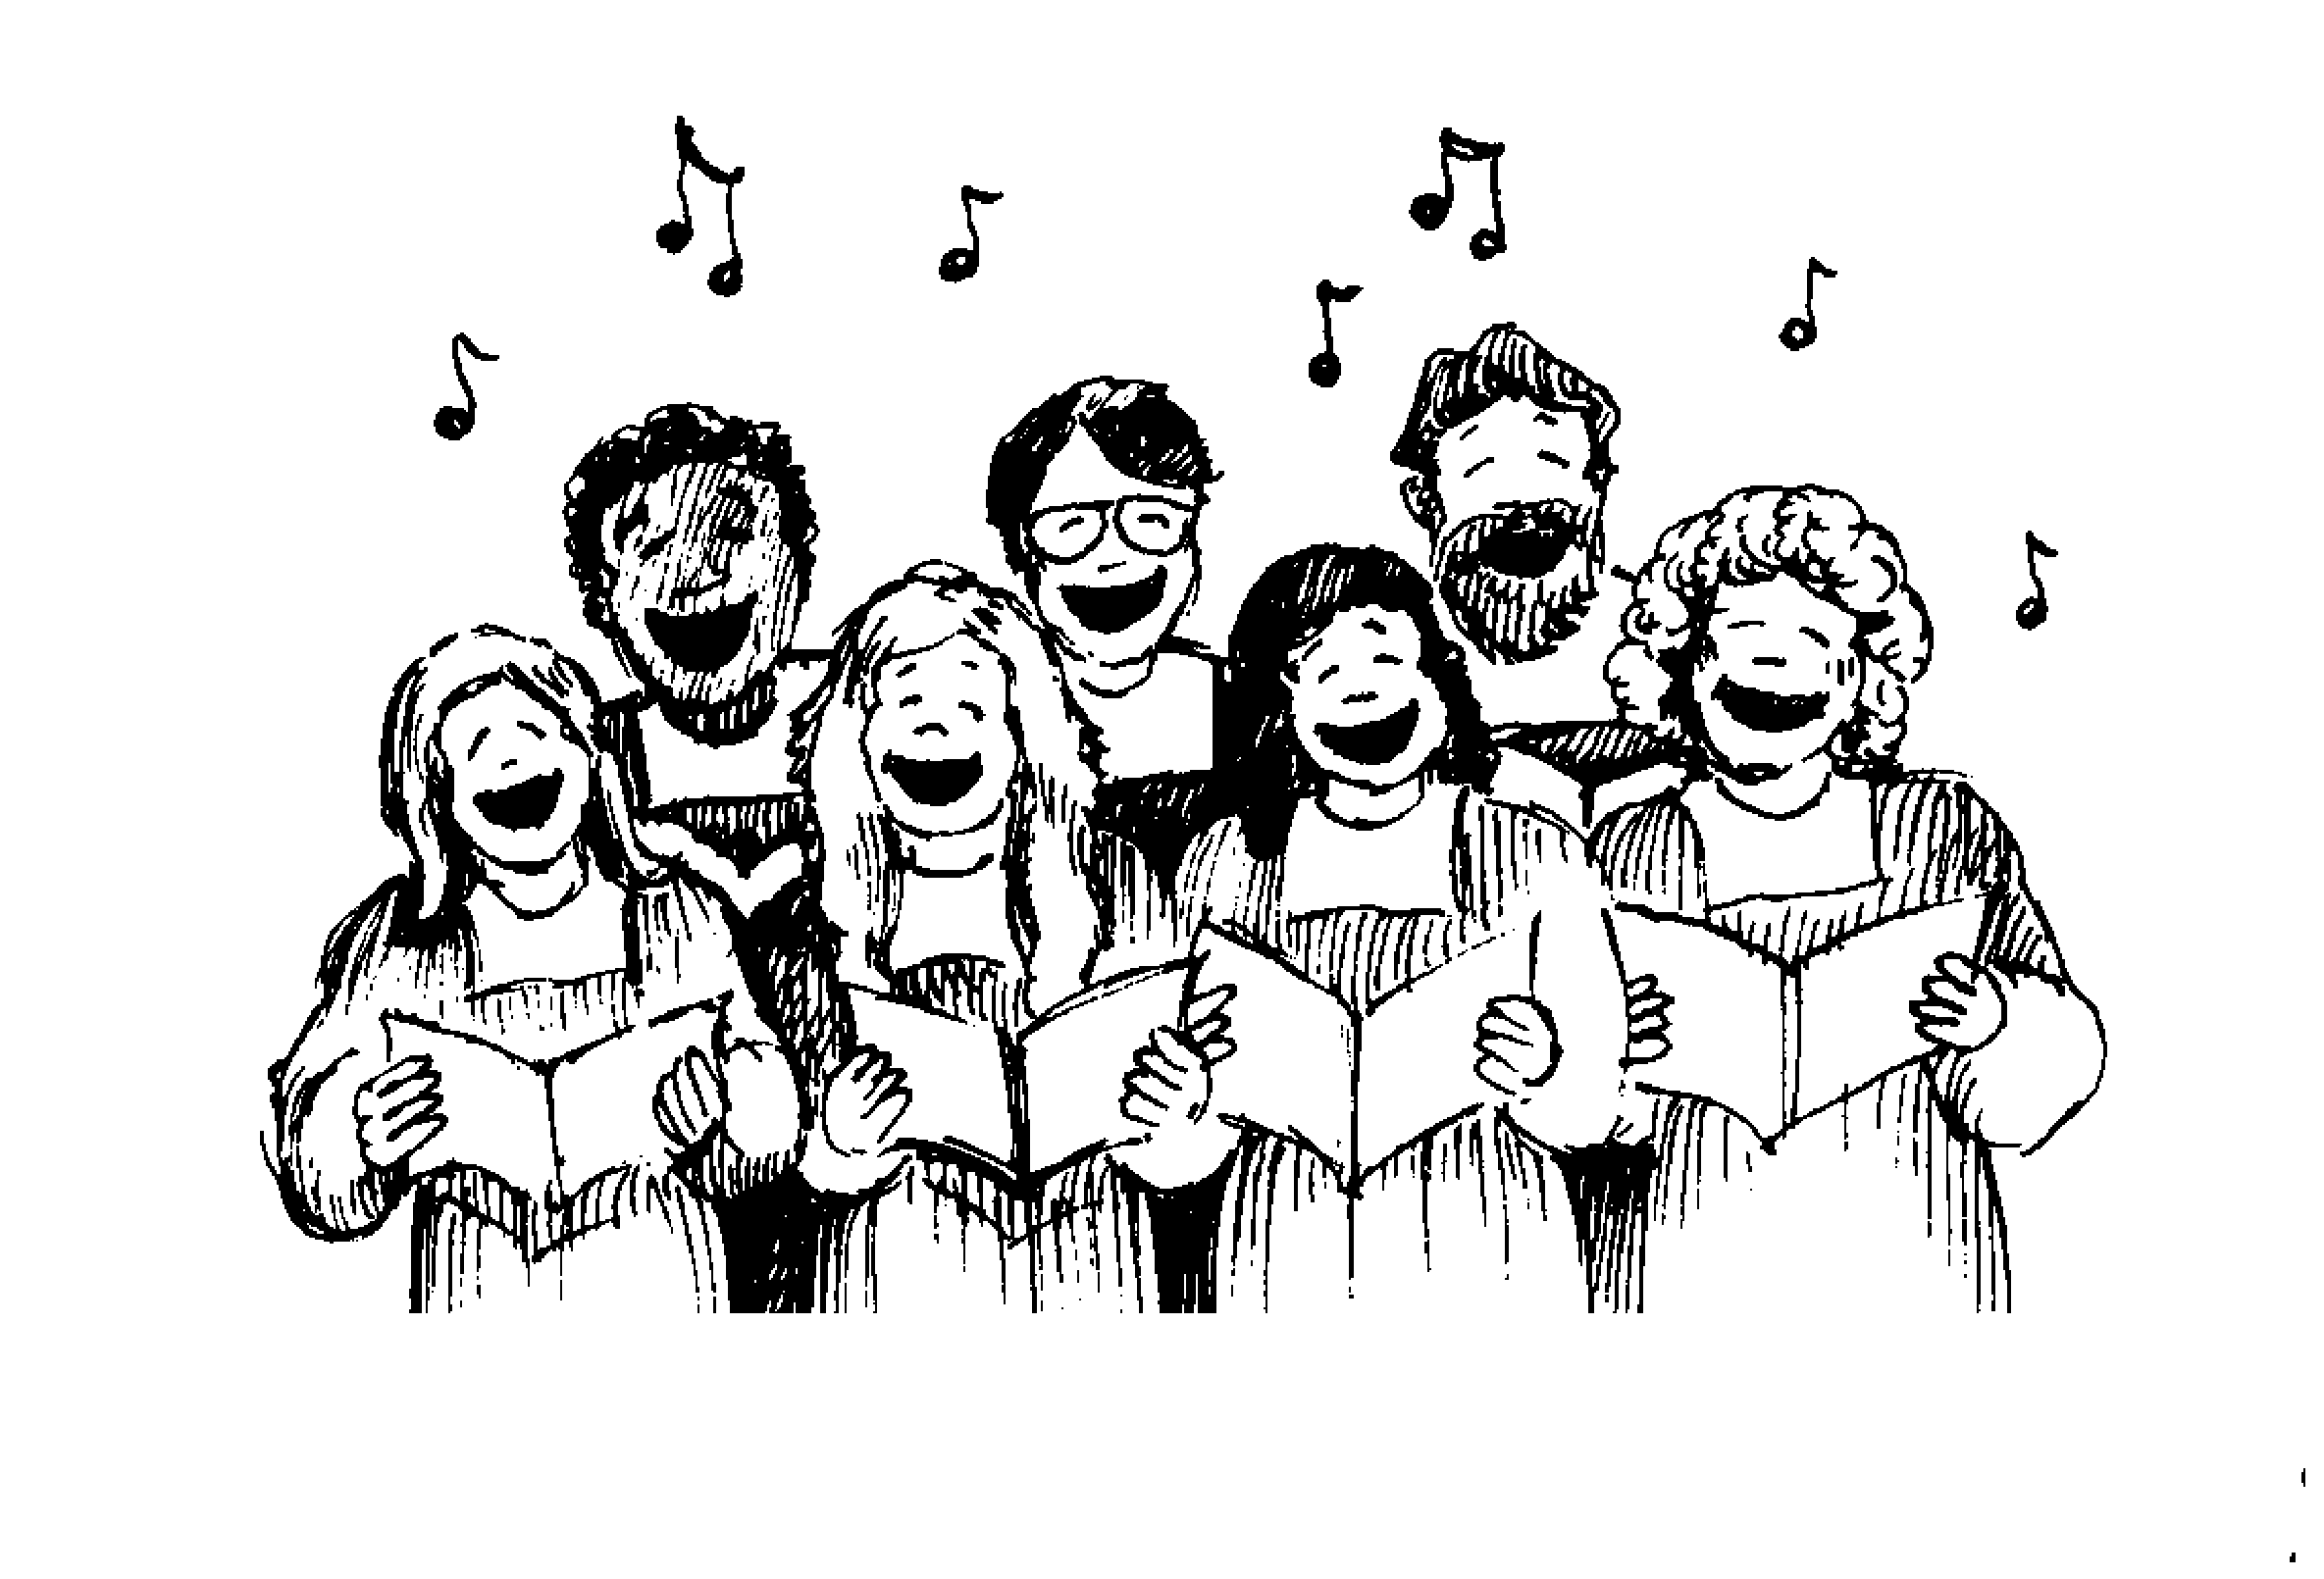
\includegraphics[scale=0.2]{choir01}
\end{center}



\end{document}